\documentclass[style=upen, size=14pt]{powerdot}
\usepackage{natbib}
\usepackage{bibentry}
\usepackage{mathtools}
\definecolor{arany}{RGB}{255,242,0}
\hypersetup{backref=page}
\hypersetup{
    colorlinks=true,
    linkcolor=cyan,
    citecolor=cyan,
    filecolor=magenta,      
    urlcolor=cyan}
% \pdsetup{trans=Split}
\usepackage{graphicx}
\usepackage{amsmath}
\DeclareMathOperator*{\argmax}{argmax}
\DeclareMathOperator*{\argmin}{argmin}
\DeclareMathOperator*{\softmax}{softmax}
\DeclareMathOperator{\sign}{sign}
\usepackage{amssymb}
\usepackage{stmaryrd}
\usepackage[latin2]{inputenc}
%\usepackage[magyar]{babel}
%\usepackage{euler}
\usepackage{tikz}
\usetikzlibrary{matrix}
%\usepackage{tikz-qtree}
%\usepackage{tikz-dependency}
%\usepackage{linguex}
\usepackage{amsthm}
\usepackage{amsmath}
%\tikzset{every tree node/.style={align=center,anchor=north}}
%\usepackage{tabularx}
%\usepackage{threeparttable}
%\usepackage{color}
%\selectlanguage{english}
%\frenchspacing
\usepackage{algpseudocode}
\usepackage{algorithm}
\newcommand\varlist{,\makebox[1em][c]{.\hfil.\hfil.},}
\newcommand{\nd}{\noindent}
\newcommand{\Val}{\mathop{\mathit{Val}}}
\newcommand{\gold}{\color{arany}}
%\usepackage{tikz}
%\usepackage{tikz-qtree}
%\newcommand{\qed}{\hfill\mbox{\raggedright \rule{.1in}{.1in}}}
\def\es{\mathbin\land}
\theoremstyle{definition}
\newtheorem*{definition}{Definition}
\newtheorem{axioma}{Axiom}
\newtheorem{tetel}{Theorem}
\newtheorem{prop}{Proposition}
\newtheorem{lemma}{Lemma}
\begin{document}

\title{Natural Language Processing\\~~\\Lecture 10\\RNN sequence models and
  attention}
% \author{}

\date{2021}
\maketitle

\begin{slide}[toc= RNN seq processing]{Sequence processing with RNNs}
  Depending on the way inputs, outputs and hidden/cell states are handled, RNNs
  can be used for a variety of sequence transformation and processing tasks:
  \begin{center}
    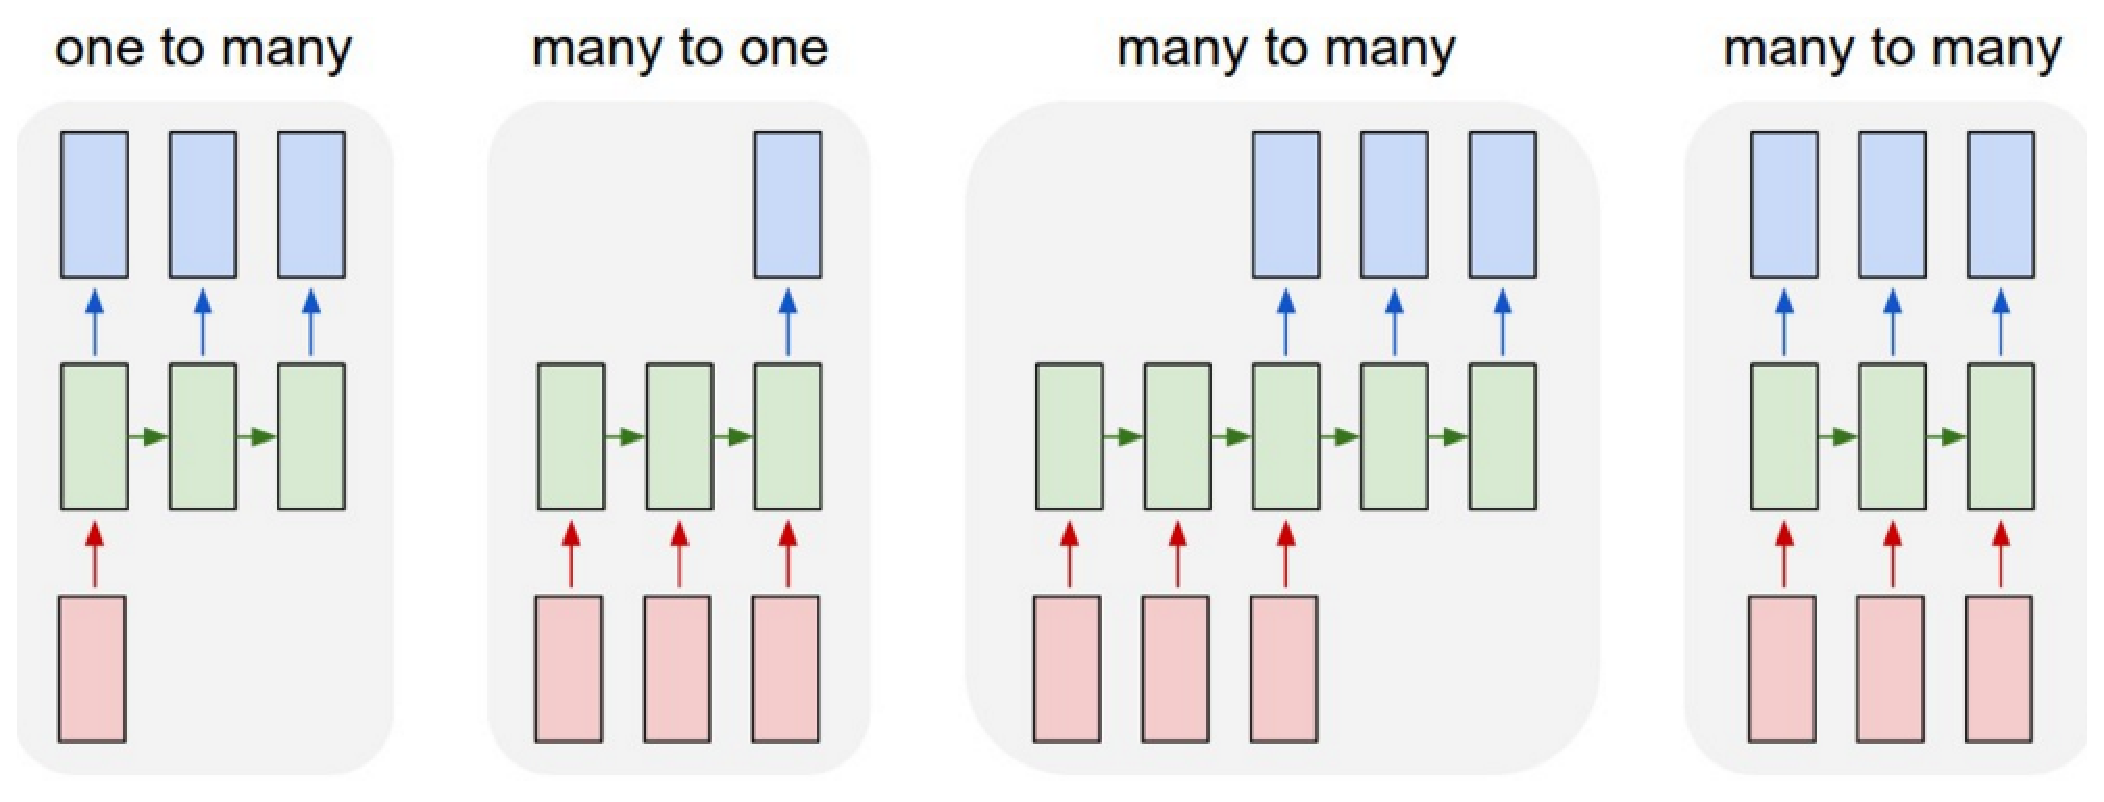
\includegraphics[width=1\textwidth]{figures/rnn_topologies.eps}
    \footnotesize{(Figure from \cite{karpathy2015unreasonable}).}
  \end{center}
\end{slide}

\begin{slide}[toc=]{Sequence processing with RNNs cont.}
  Perhaps the most basic is the many-to-many transformation of an
  $\langle \mathbf{x}_1,\dots,\mathbf{x}_n \rangle$ input sequence to the
  $\langle \mathbf{y}_1,\dots,\mathbf{y}_n\rangle$ sequence of corresponding
  outputs at each time step.

  This type of architecture can be used e.g., for sequence tagging, when the
  outputs are distributions over the tags. Language modeling can be considered a
  special case of sequence tagging, when the correct ``tag'' of each word in a text is
  simply the next word:
  $$
  \mathbf{x} = \langle w_1,\dots,w_{n-1}\rangle,
  $$
  $$
  \mathbf{y} = \langle w_2,\dots,w_{n}\rangle.
  $$
\end{slide}

\begin{slide}{Sequence tagging}
  A simple tagging example: LSTM-based POS-tagger with word-embedding input and
  softmax output layers.
  \begin{center}
    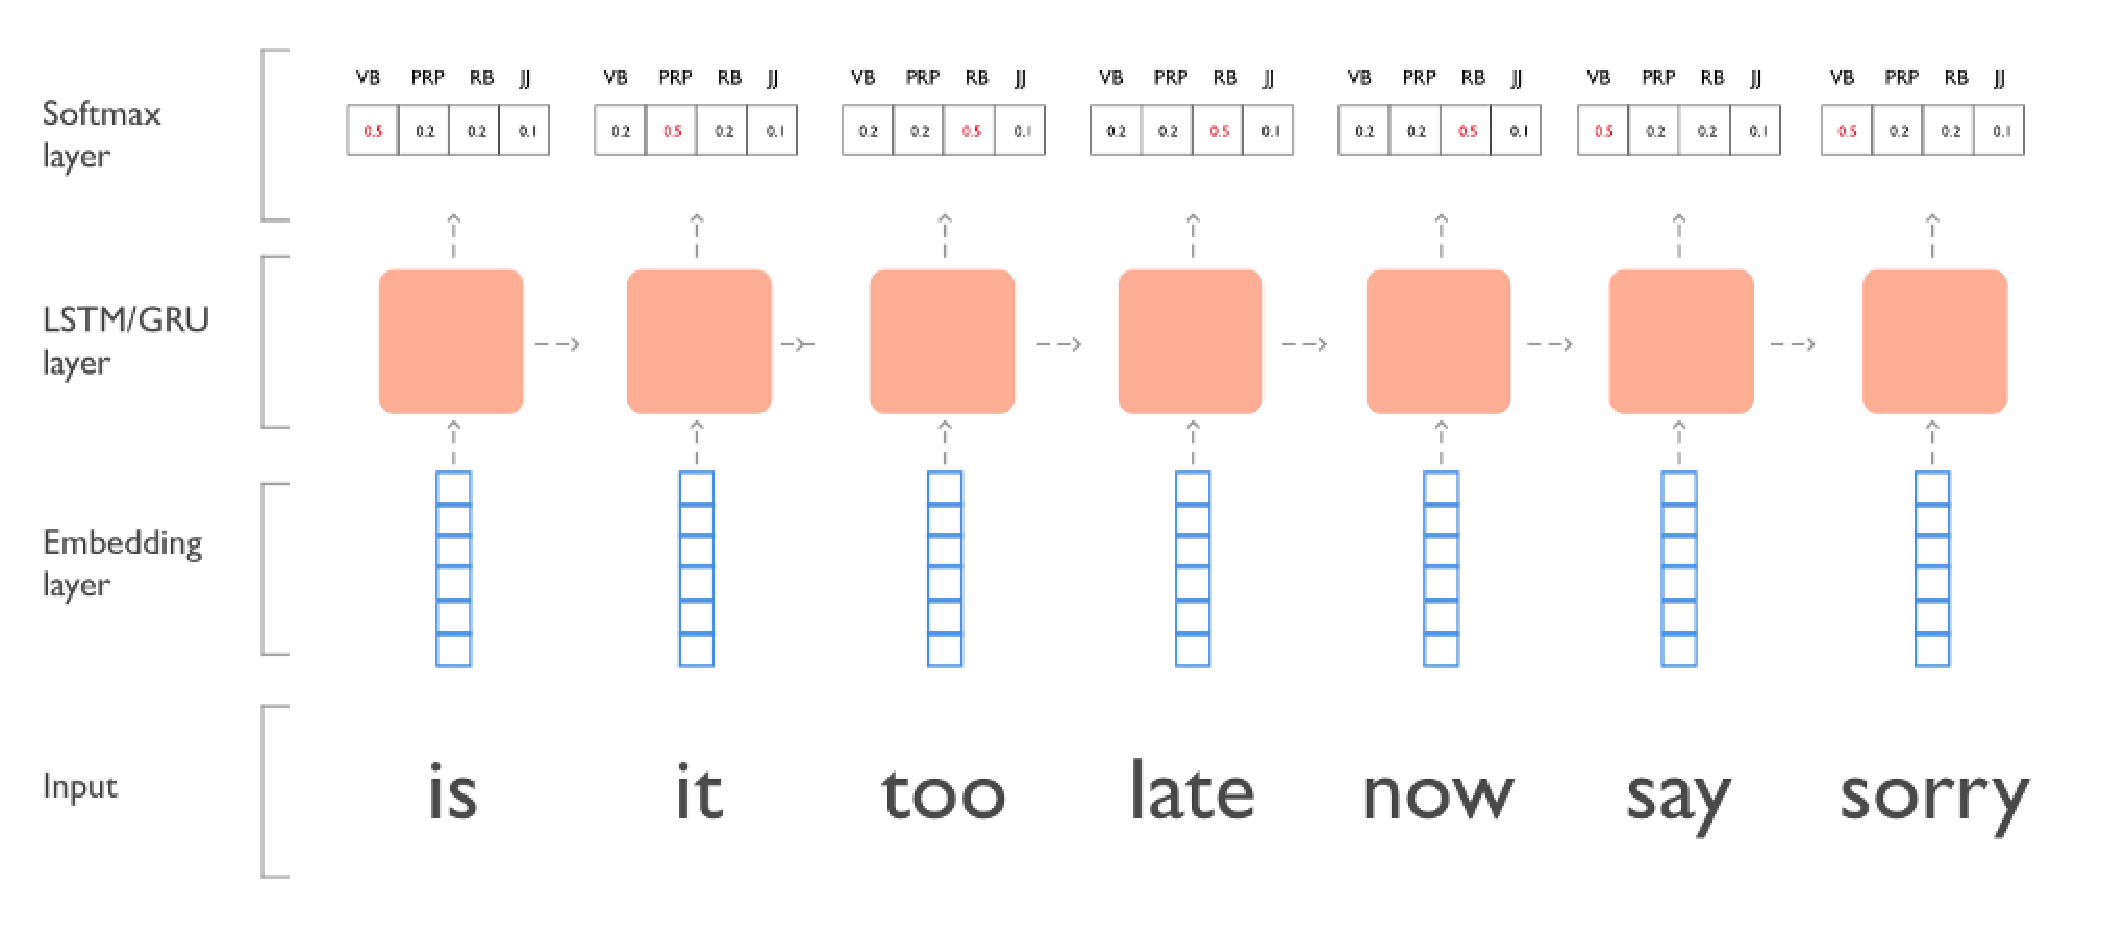
\includegraphics[width=1\textwidth]{figures/rnn_sequence_tagging.eps}
    \footnotesize{(Figure from \cite{falcon2018taming}.)}
  \end{center}
\end{slide}

\begin{slide}{Bidirectional RNNs}
  Language modeling as a sequence tagging task has a very particular property:
  models cannot have access to information about elements \emph{after} the
  element to be tagged.\bigskip

  For other sequence tagging tasks this does not hold: context \emph{after} the
  element is an important part of the input. But an RNN unit is inherently
  one-directional: hidden states can contain information only about inputs at
  earlier time steps. A widespread way of providing access to the full context
  is using RNNs in \emph{both directions} and concatenate their hidden states at
  each element. This is a so-called \emph{\gold bidirectional RNN} layer.
\end{slide}

\begin{slide}[toc=]{Bidirectional RNNs cont.}
    \begin{center}
    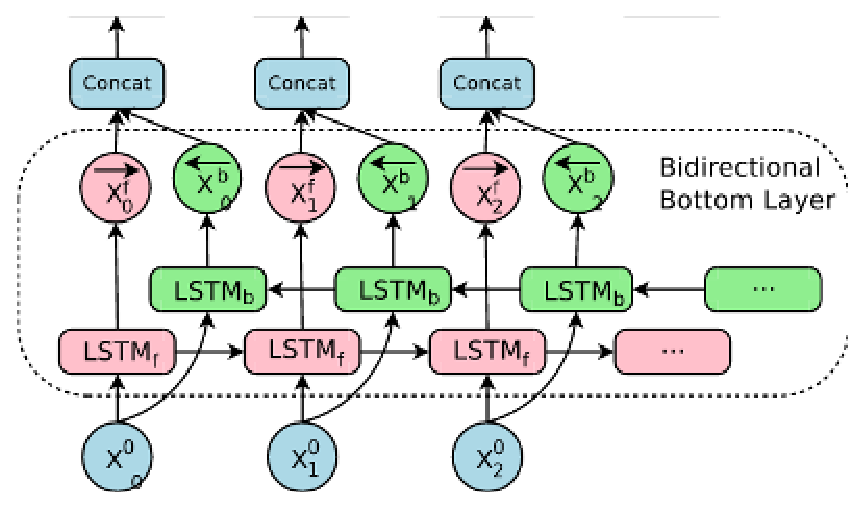
\includegraphics[width=0.85\textwidth]{figures/birnn.eps}
  \end{center}
  Naturally, bidirectional RNN layers can be stacked similarly to ordinary,
  one-directional RNNs.
\end{slide}

\begin{slide}[toc=Sequence encoding]{Seq2vec: sequence encoding}
  There are many tasks for which a variable-length input sequence has to be
  mapped to a fixed-length output, e.g., sequence classification tasks like
  sentiment classification.\bigskip

  How can one or several stacked RNNs be used to map the input sequence to a
  vector which is a useful representation of the whole input? The key is that
  RNN \emph{hidden states} (plus the cell states of LSTMs) can
  represent the whole input sequence up to the given time step.
\end{slide}

\begin{slide}[toc=]{Seq2vec: sequence encoding cont.}
  In the case of one-directional RNN(s), the obvious solution is to use the
  \emph{last hidden state} (possibly together with the cell state in case of
  LSTMs) to represent the whole input sequence. E.g., for classification:
  \begin{center}
    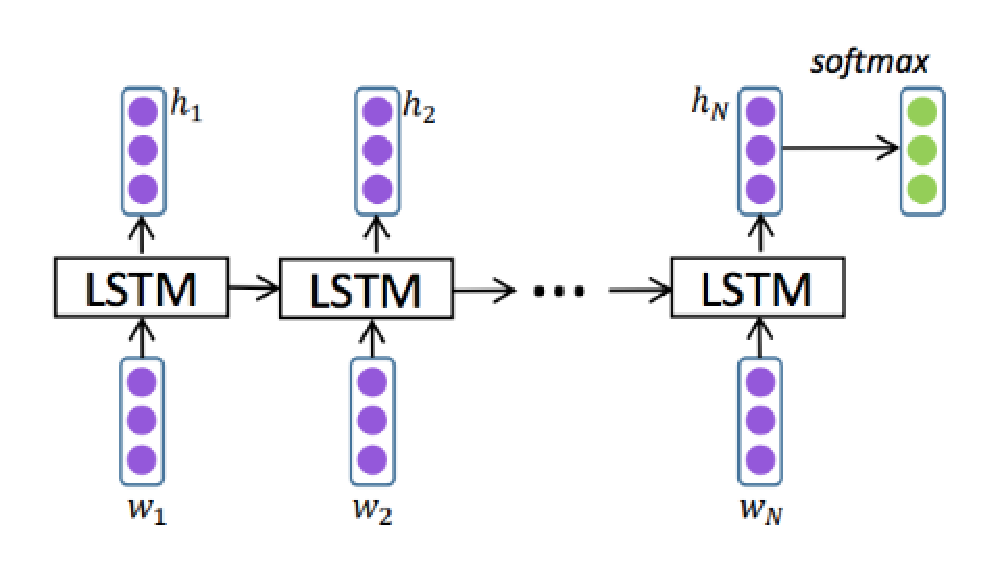
\includegraphics[width=0.7\textwidth]{figures/seq2vec.eps}
    
    \footnotesize{(Figure from \cite{minaee2019deep}.)}
  \end{center}
\end{slide}

\begin{slide}[toc=]{Seq2vec: sequence encoding cont.}
  The (combined) hidden states of bi-RNNs, in contrast, contain information
  about the entire input at each time step, so it makes more sense to aggregate
  all of them, e.g., by taking their average or using max pooling.
    \begin{center}
    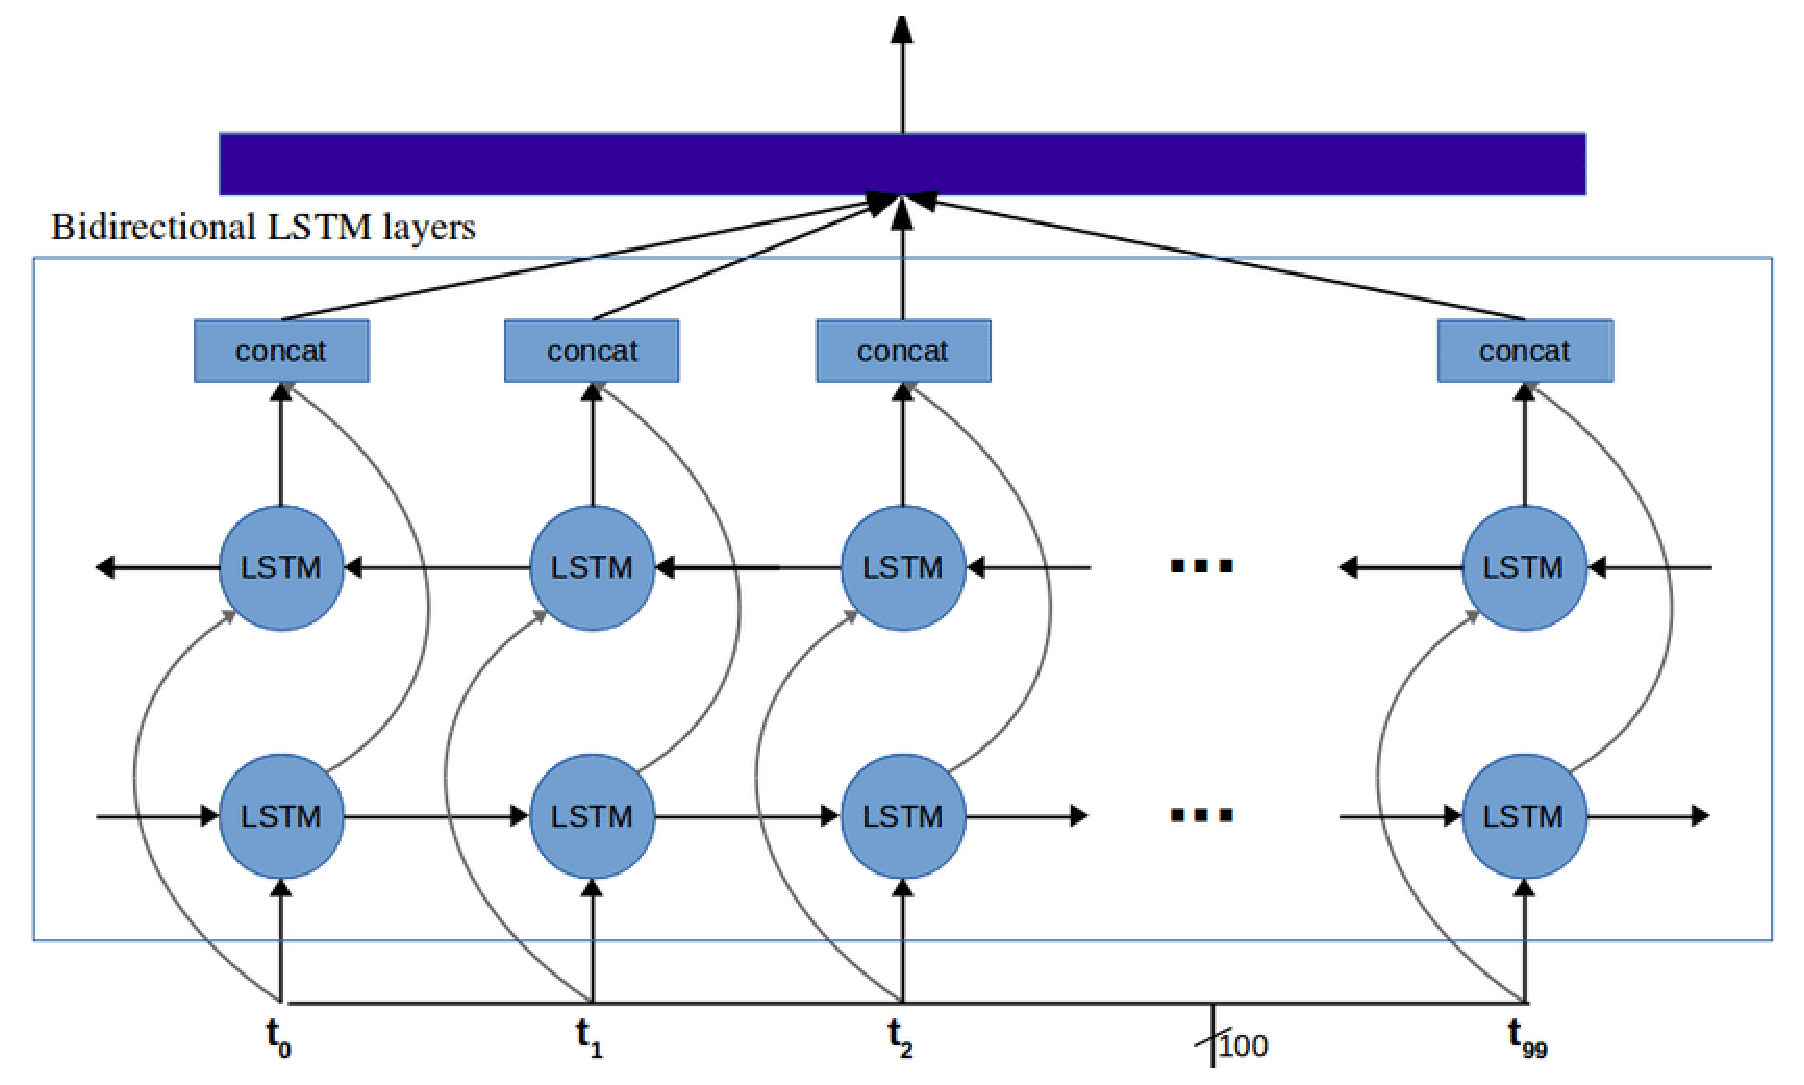
\includegraphics[width=0.7\textwidth]{figures/birnn_aggregation.eps}
    
    \footnotesize{(Figure adapted from \cite{faust2018automated}.)}
  \end{center}
\end{slide}

\begin{slide}[toc=Sequence generation]{Vec2seq: sequence generation}
  Sequence generation based on a fixed size vector is analogous to language
  generation with a language model, but in this case generation is
  \emph{conditional}: we want to model sequence probabilities
  $$
  P(\langle y_1,\dots, y_n\rangle ~|~ \mathbf{x}) 
  $$
  where $\mathbf{x}$ is a fixed length vector. Similarly to RNN-based
  \emph{uncoditional} language models, we can reduce the problem to modeling the
  individual
  $$
  P( y_n|~ \langle y_1,\dots,y_{n-1} \rangle, \mathbf{x})
  $$
  \emph{continuation probabilities} with RNNs.
\end{slide}

\begin{slide}[toc=]{Vec2seq: sequence generation cont.}
  The standard RNN-based language model architecture can be reused with a single
  modification: the RNN hidden states are also conditioned on the condition
  vector $\mathbf{x}$. The model has the following conditional independence
  structure:
  \begin{center}
    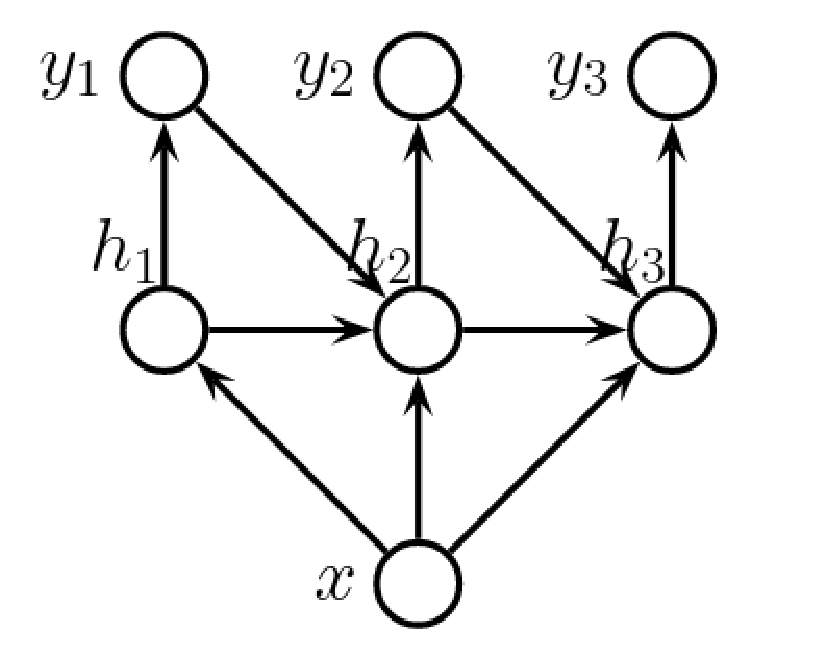
\includegraphics[width=0.45\textwidth]{figures/vec2seq_graph_mod.eps}
    
    \footnotesize{(Figure from \cite{murphy2021pml}.)}
  \end{center}
\end{slide}

\begin{slide}[toc=]{Vec2seq: sequence generation cont.}
  On the neural architecture level, conditioning the RNN hidden states on 
  $\mathbf{x}$ can be implemented in several ways:
  \begin{itemize}
  \item use $\mathbf{x}$ (directly or after a transformation) as the
    \emph{initial hidden state} of the RNN (also as the initial cell state for
    LSTMs);
  \item use $\mathbf{x}$ (directly or transformed) as the \emph{input} at the
    \emph{first time step};
  \item use $\mathbf{x}$ (directly or transformed) as the \emph{input} at
    \emph{each time step} (in addition to the already generated sequence
    elements).
  \end{itemize}
\end{slide}

\begin{slide}[toc=]{Vec2seq: sequence generation cont.}
  The first two solutions are the most widely used, e.g., the following image
  captioning model uses the image's feature vector as the first LSTM
  input:\medskip
  
  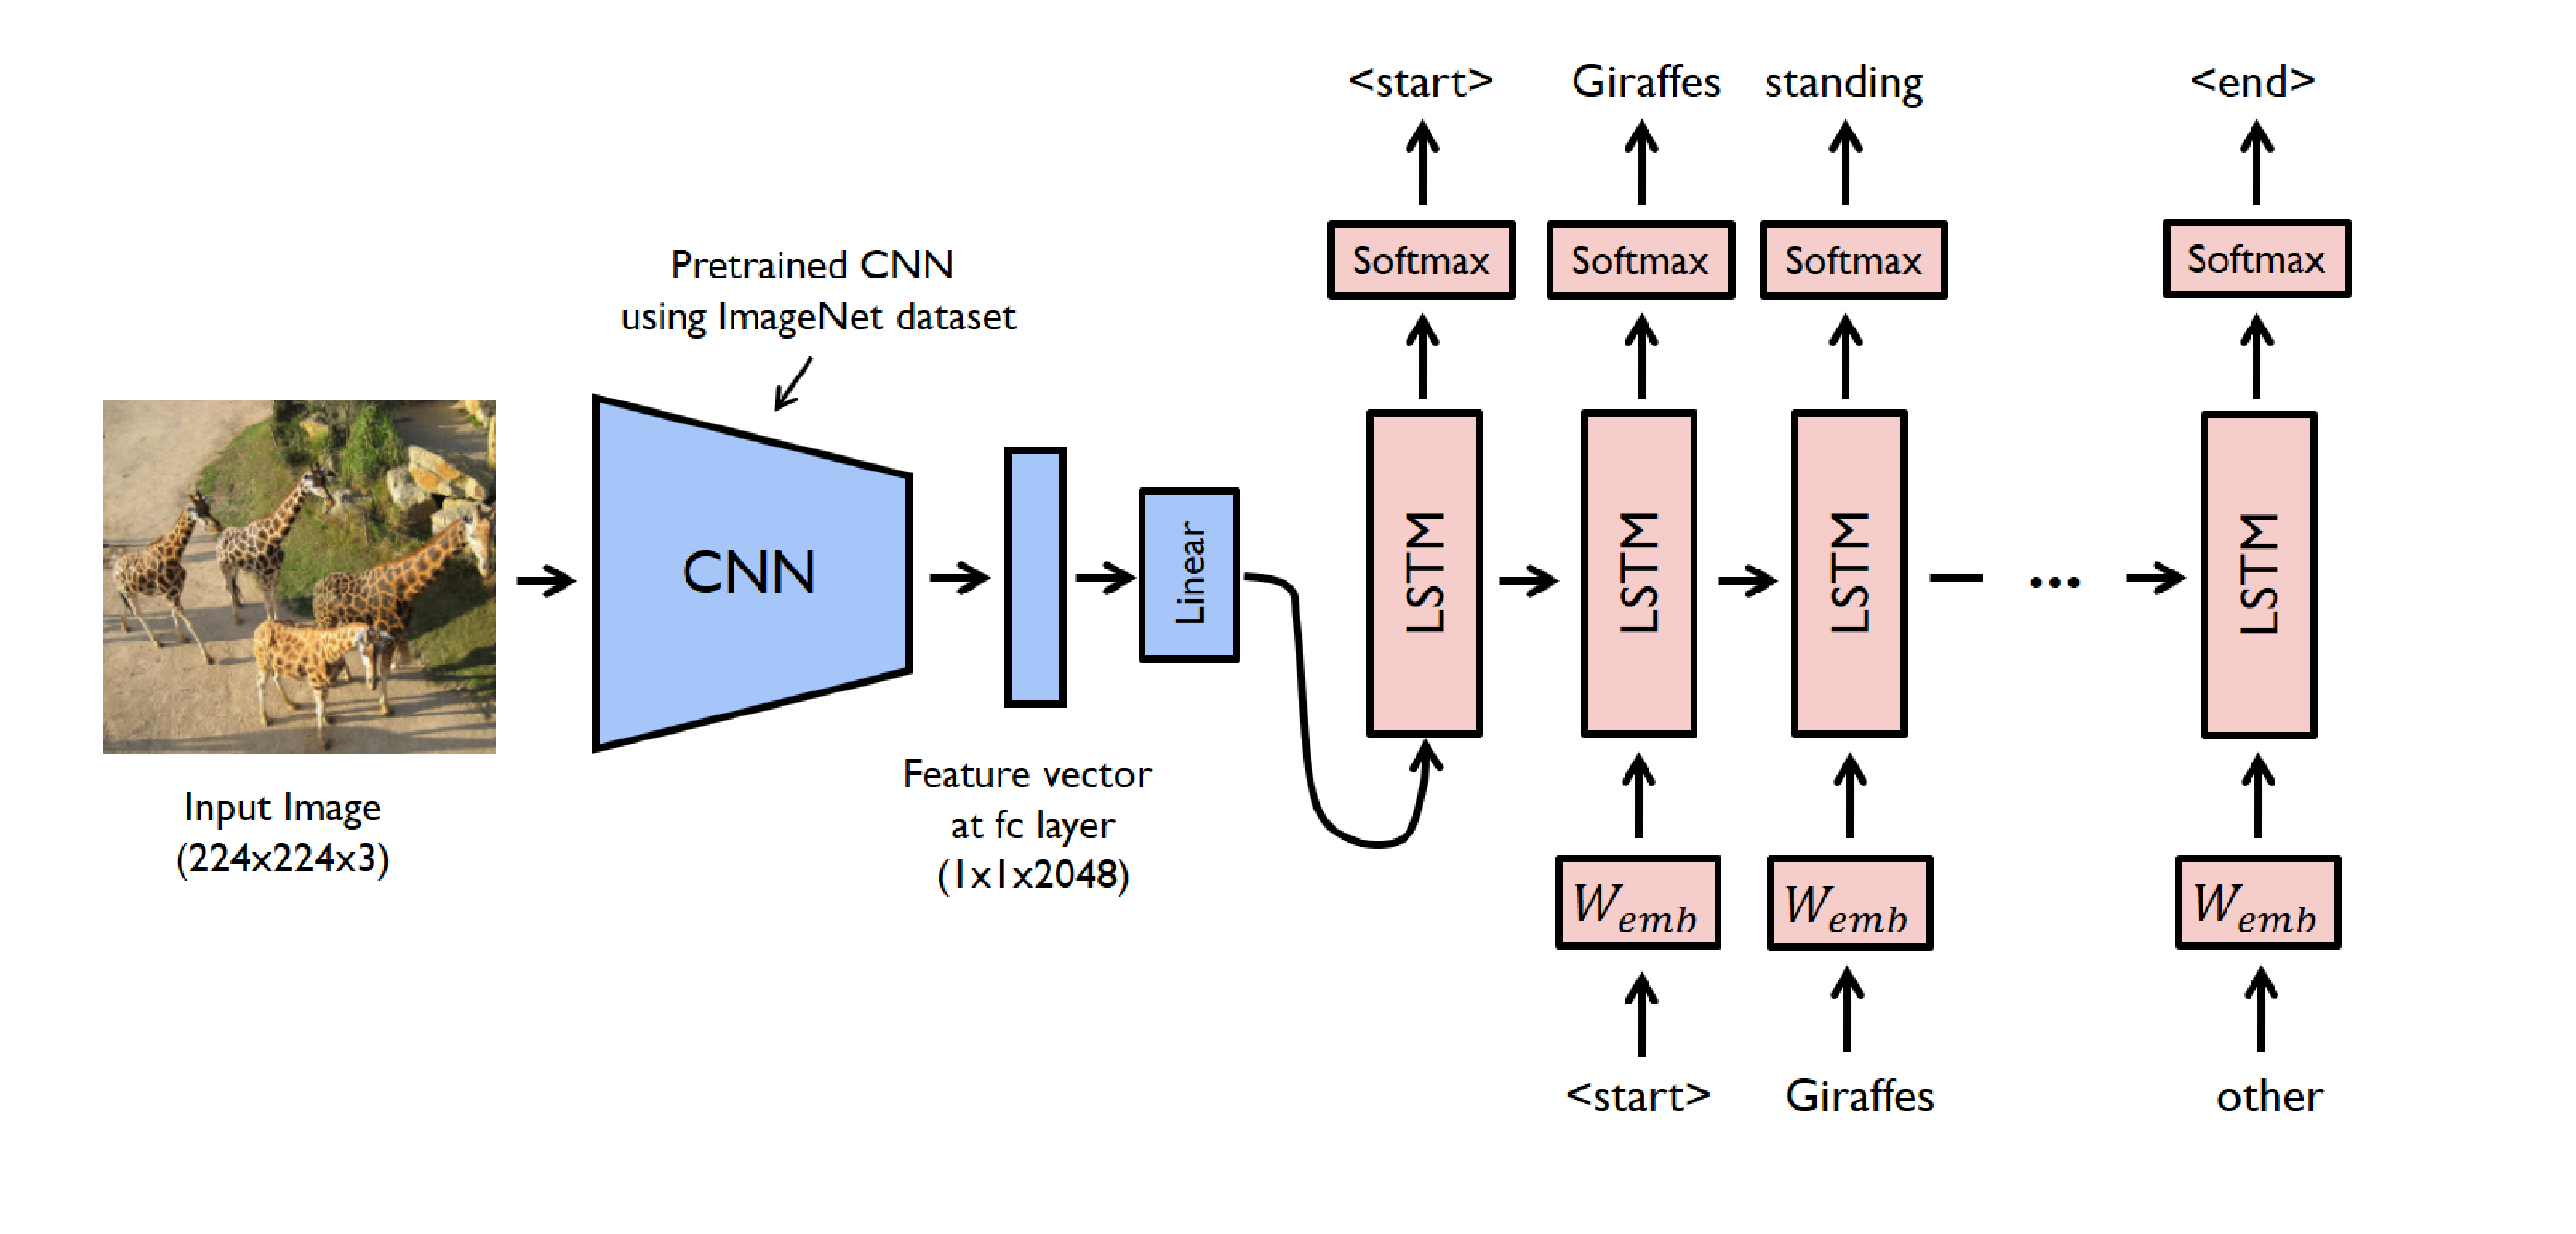
\includegraphics[width=1.\textwidth]{figures/image_captioning.eps}
  
  \hspace{2.6cm}\footnotesize{(Figure from Yunjey Choi's
    \href{https://github.com/yunjey/pytorch-tutorial/tree/master/tutorials/03-advanced/image_captioning}{PyTorch
      tutorial}.)}
\end{slide}

\begin{slide}[toc=]{Vec2seq: sequence generation cont.}
  The training of Vec2seq models is, again, analogous to that of unconditional
  language models:
  \begin{itemize}
  \item The dominant strategy is \emph{teacher forcing}: the training dataset's
    sequences are used as RNN input, the predicted continuation probabilities
    are used only for calculating the loss (negative log likelihood).
  \item As in the unconditional case, teacher forcing leads to \emph{exposure
      bias} (an unhealthy gap between the training and inference setting), so
    alternative training strategies such as \emph{scheduled sampling} are also
    used.
  \end{itemize}
\end{slide}

\begin{slide}{RNN-based Seq2seq}
  By combining an RNN Seq2vec with an RNN Vec2seq module we can build a Seq2seq
  model which transforms a variable-length input sequence into another
  \emph{unaligned} sequence by first \emph{\gold encoding} the input into a
  fixed-size vector representation and then \emph{\gold decoding} this vector
  into another sequence. The probabilistic structure of the combined model is:
  \begin{center}
    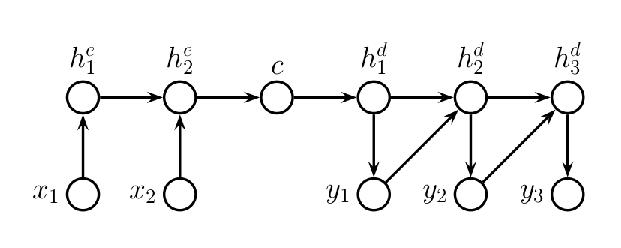
\includegraphics[width=0.7\textwidth]{figures/seq2seq_prob.eps}
    
    \footnotesize{(Figure from \cite{murphy2021pml}.)}
  \end{center}
\end{slide}

\begin{slide}[toc=]{RNN-based Seq2seq cont.}
  Historically, RNN-based Seq2seq models were among the most successful
  applications of RNNs (more concretely, of LSTM variants). Applications
  included

  \begin{itemize}
  \item machine translation (LSTM Seq2seq models were the first neural MT models
    competitive with and later superior to traditional phrase-based solutions),
  \item summarization,
  \item question answering, and
  \item dialogue systems.
  \end{itemize}
\end{slide}

\begin{slide}[toc=]{RNN-based Seq2seq cont.}
  Architecturally, these models are typically
  \begin{itemize}
  \item embedding-based,
  \item use several LSTM layers in both the encoder and the decoder,
  \item initialize the hidden state and the cell state of the decoder with the
    (last or aggregated) hidden states and cell states of the encoder,
  \item are trained, as usual, with teacher forcing and negative log likelihood
    loss.
  \end{itemize}
  While the decoder cannot contain backward RNNs (for obvious reasons), the
  encoder often contains bidirectional RNN layers.
\end{slide}

\begin{slide}[toc=]{RNN-based Seq2seq cont.}
  A typical machine translation model:
    \begin{center}
    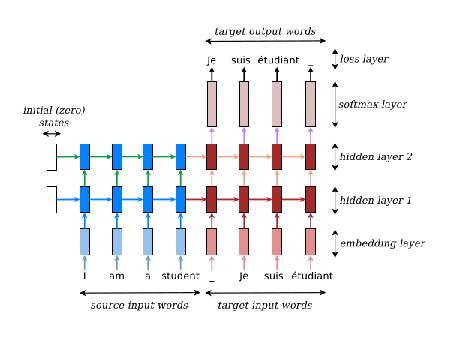
\includegraphics[width=0.7\textwidth]{figures/seq2seq_trans.eps}
    
    \footnotesize{(Figure from \cite{luong2016neural}.)}
  \end{center}
\end{slide}

\begin{slide}{Attention}
  In basic RNN Seq2seq models, as we have seen, the decoder could access the
  encoded input sequence only in the form of the fixed-size vector
  representation(s) produced by the encoder.\bigskip

  Significantly, this fixed-size ``summary'' did not depend on \emph{where} the
  decoder was in the decoding process, even though we know that for typical
  Seq2seq tasks, e.g. for translation, different parts of the input are relevant
  at different decoding stages.

  Even if the fixed size vector was produced by pooling the whole sequence of
  encoder hidden states, the decoder's context has no influence on the pooling.
\end{slide}

\begin{slide}[toc=]{Attention cont.}
  Attention mechanisms solve the problem by providing access to
  \emph{dynamically pooled} versions of the encoder hidden states at each
  decoding time step, \emph{based on the encoder's context}, i.e., the
  $h_{t-1}^d$ hidden state:
  \begin{center}
    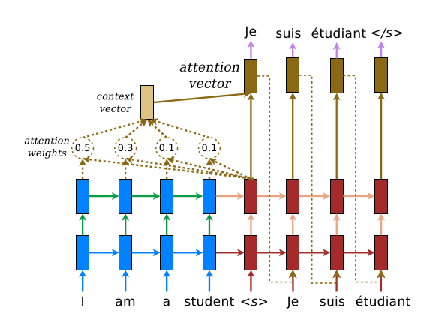
\includegraphics[width=0.55\textwidth]{figures/seq2seq_attention}
    
    \footnotesize{(Figure from \cite{luong2016neural}.)}
  \end{center}
\end{slide}

\begin{slide}[toc=]{Attention cont.}
  Concretely, attention mechanisms \emph{score} the
  $\mathbf{h}^e=\langle h_1^e\dots,h_n^e \rangle$ encoder hidden states based on
  the $h^d_{t-1}$ decoder context using an $s(\cdot, \cdot)$ scoring function, and
  produce a weighted sum with the softmax of the scores:
  $$
  \mathbf{s}(\mathbf{h}^e, h_{t-1}^d ) =\langle s({h}^e_1, h_{t-1}^d),\dots,
  s({h}^e_n, h_{t-1}^d) \rangle,
  $$
  
  $$
  \mathcal A(\mathbf{h}^e, h_{t-1}^d) =  \softmax(\mathbf{s}(\mathbf{h}^e, h_{t-1}^d )) \cdot \mathbf{h}^e.
  $$
\end{slide}

\begin{slide}[toc=]{Attention: scoring functions}
  There are two main types of attention according to the type of scoring
  function they use:
  \begin{itemize}
  \item \emph{\gold Additive} or \emph{\gold MLP} or \emph{\gold Bahdanau}
    attention: the score is calculated by a simple feedforward network with one
    hidden layer:
    \begin{small}
      $$
      s_{add}(\mathbf{a}, \mathbf{b}) =
      \mathbf{v^\intercal}\tanh(\mathbf{W_1\mathbf{a} + \mathbf{W_2} \mathbf{b}}),
      $$
    \end{small}
    where $\mathbf{v}$, $\mathbf{W}_1$ and $\mathbf{W}_2$ are learned 
    parameters.
  \item \emph{\gold Multiplicative} or \emph{\gold Luong} attention: the score
    is calculated as
    \begin{small}
      $$
      s_{mult}(\mathbf{a}, \mathbf{b}) =
      \mathbf{a}^{\intercal} \mathbf{W} \mathbf{b},
      $$
    \end{small}
    where $\mathbf{W}$ is, again, learned.
  \end{itemize}
\end{slide}

\begin{slide}[toc=]{Dot product attention}
  \emph{\gold Dot product} scoring is an important, simple multiplicative
  scoring variant, in which $\mathbf{W}$ is identity, i.e.,
  $$
  s_{dot}(\mathbf{a}, \mathbf{b}) = \frac{\mathbf{a} \cdot \mathbf{b}}{\sqrt d},
  $$
  where $d$ is the dimensionality of $\mathbf{a}$ and $\mathbf{b}$, and the
  division with $\sqrt d$ ensures that the scores have 0 mean and 1 variance if the
  $\mathbf{a}$ and $\mathbf{b}$ inputs have.
\end{slide}

\begin{slide}[toc=]{Performance gains from attention} Adding attention
  mechanisms to RNN Seq2seq architectures typically results in sizable
  performance gains, \citet[63]{luong2016neural}, e.g., reports 11\% perplexity
  and 20\% BLEU score improvement on a translation task.\bigskip

  As a result, state-of-the-art RNN Seq2seq models virtually always contain some
  type of attention mechanism.
\end{slide}

\begin{slide}[toc=]{Performance gains from attention cont.}
  Attention weight visualizations show how they reflect relevance to the decoding step:
  \begin{center}
    \includegraphics[width=0.55\textwidth]{figures/attention_sentence.eps}
  \end{center}
\end{slide}


\begin{slide}[toc=CNNs]{Prologue: CNNs as sequence models}
  Although our discussion has concentrated on RNNs, {\gold convolutional
    networks} are rather competitive in many NLP tasks. They use 1d
  convolutions:
  \begin{center}
    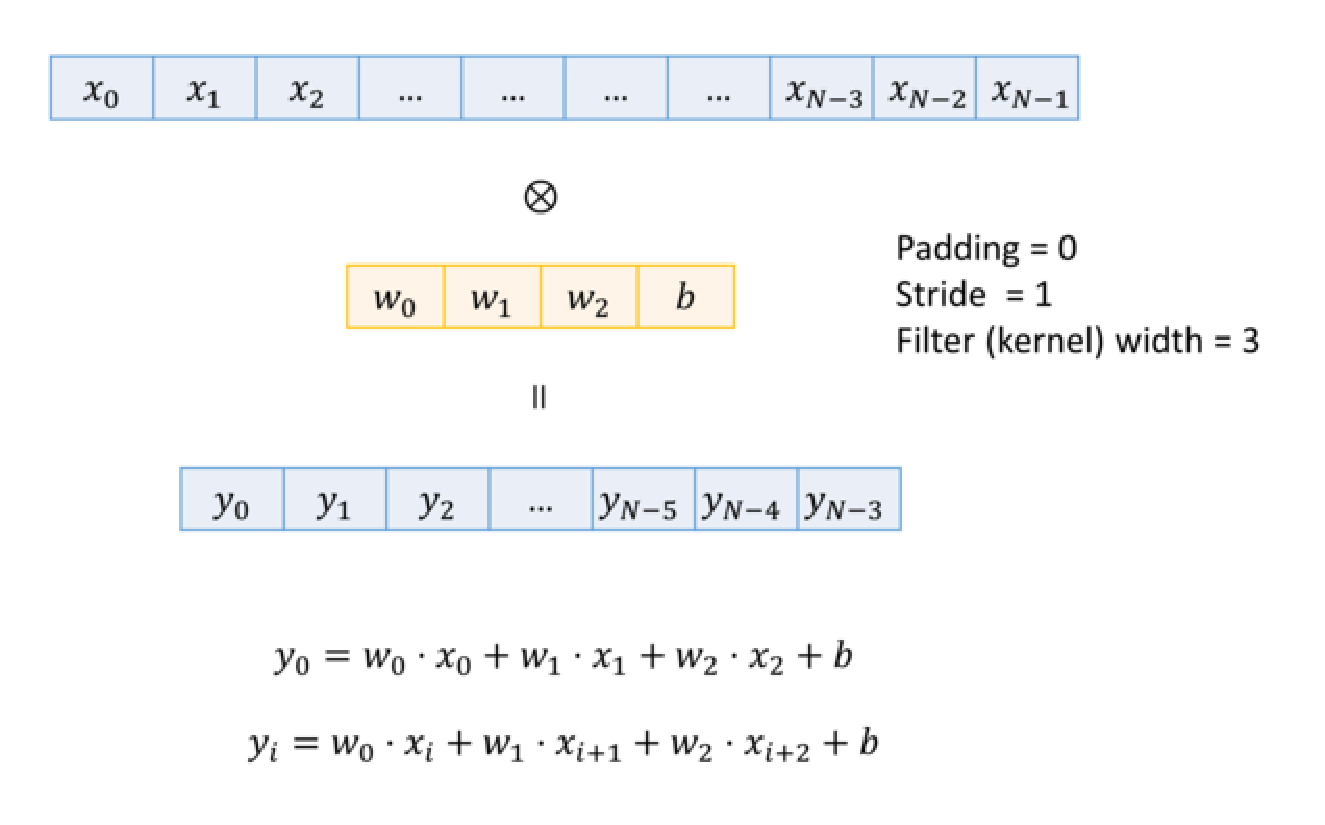
\includegraphics[width=0.8\textwidth]{figures/1d_conv.eps}
  \end{center}
\end{slide}

\begin{slide}[toc=]{Prologue: CNNs as sequence models}
  \dots and 1d (typically max- or average) pooling layers. In fact, the surprisingly
  well performing {\gold fastText} classification model uses pooling
  \emph{without} convolution:\footnote{Figure from \cite{joulin2016bag}.}
  \begin{center}
    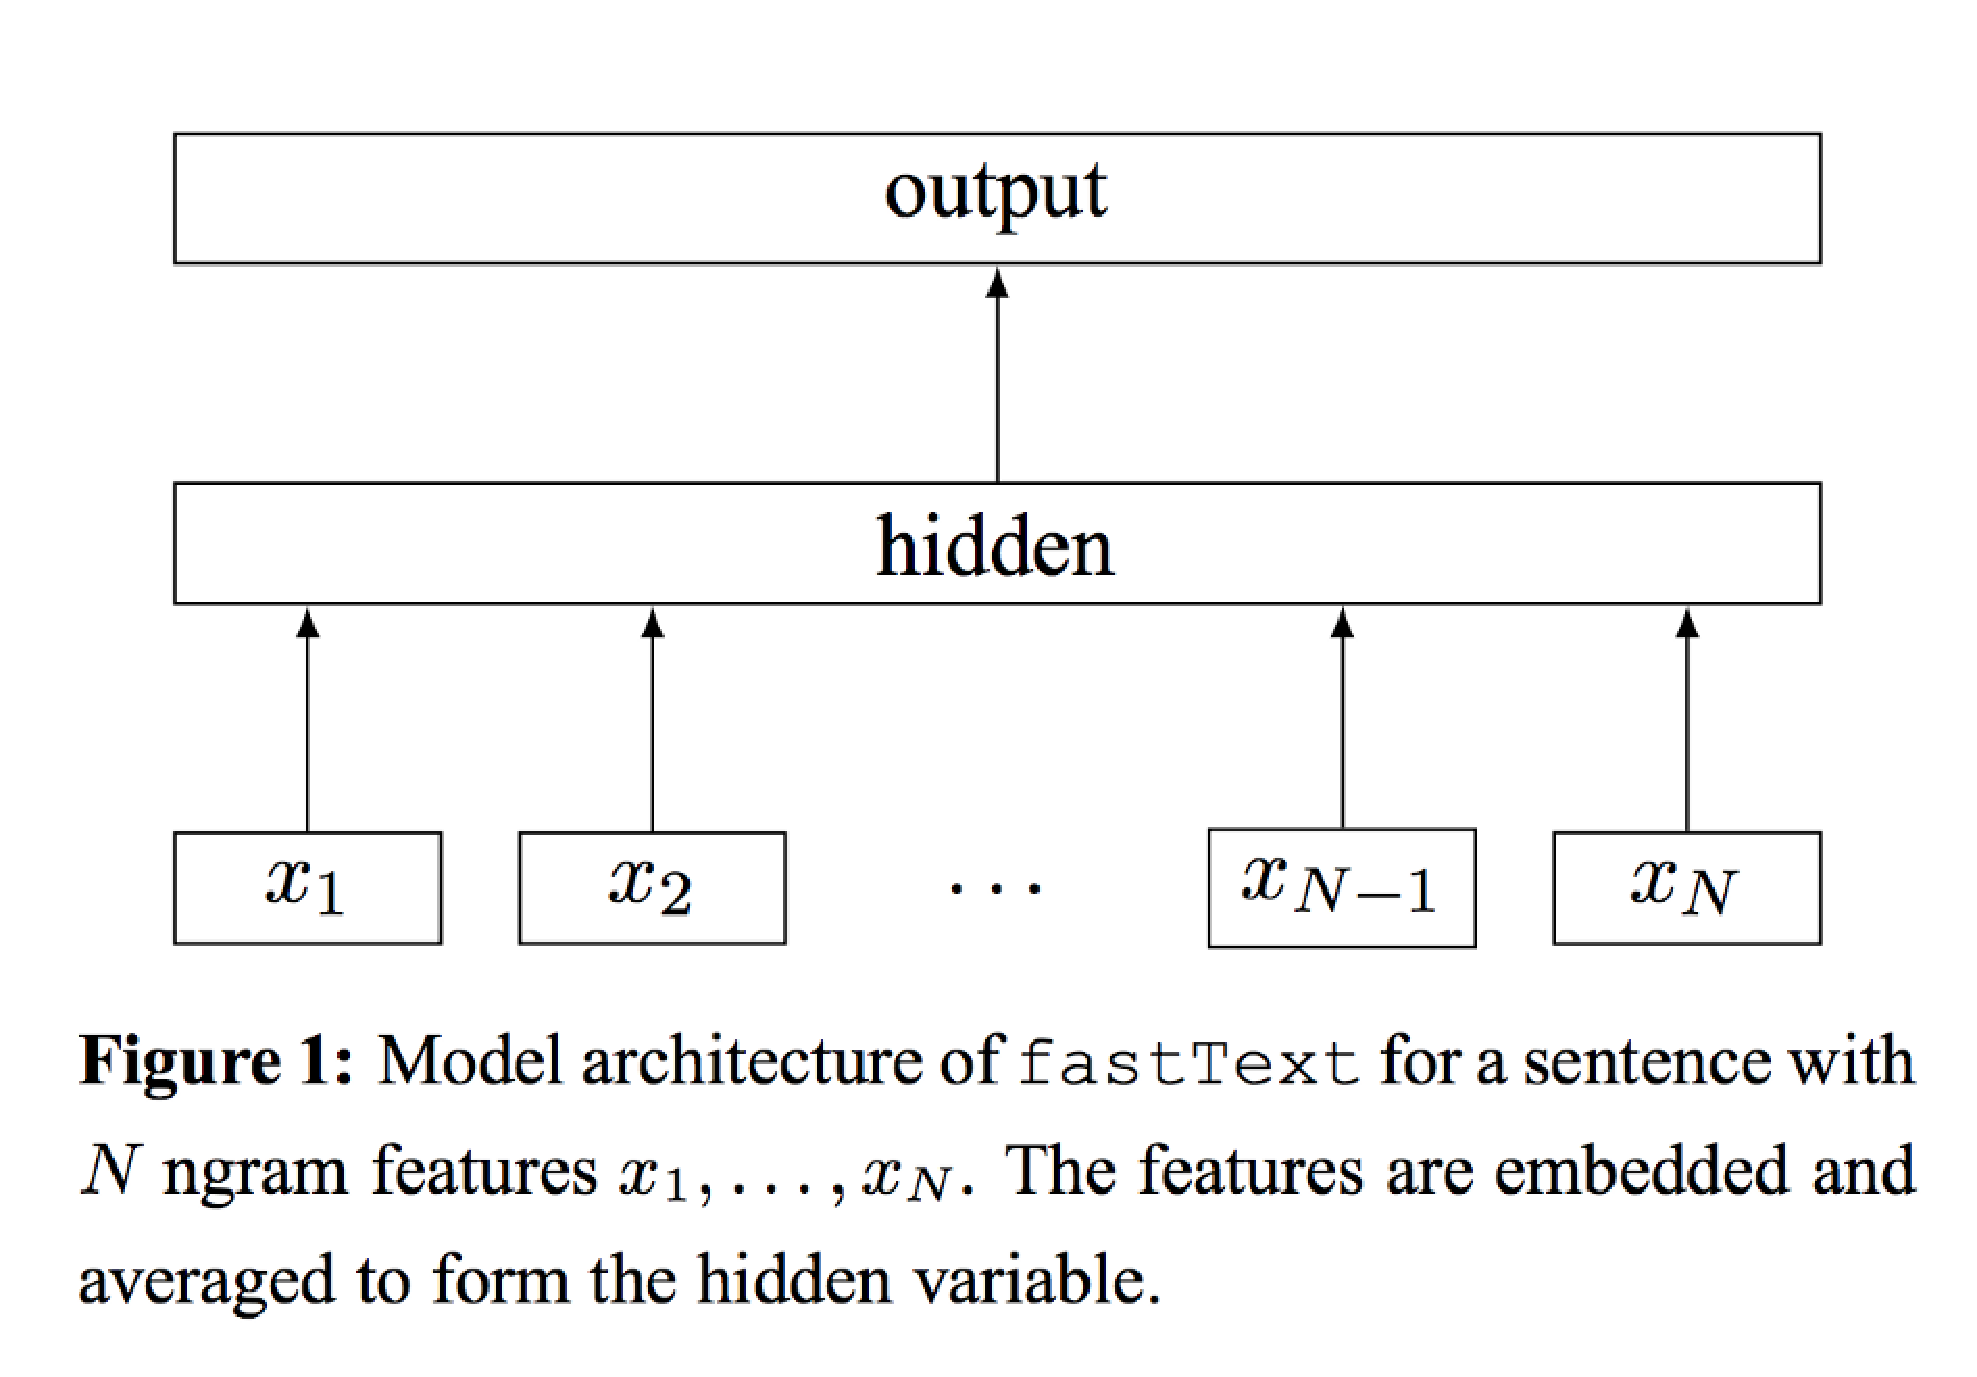
\includegraphics[width=0.65\textwidth]{figures/fastext.eps}
  \end{center}
\end{slide}

\begin{slide}{References}
  \bibliographystyle{plainnat}
  \nobibliography{nlp_course.bib}
  \begin{footnotesize}

    \bibentry{falcon2018taming}\medskip

    \bibentry{faust2018automated}\medskip
    
    \bibentry{karpathy2015unreasonable}\medskip

    \bibentry{joulin2016bag}\medskip

    \bibentry{luong2016neural}\medskip

  \end{footnotesize}
\end{slide}

\begin{slide}[toc=]{References cont.}
  \begin{footnotesize}

    \bibentry{minaee2019deep}\medskip
    
    \bibentry{murphy2021pml}\medskip
    
  \end{footnotesize}
\end{slide}

\end{document}

%%% Local Variables:
%%% mode: latex 
%%% TeX-master: t
%%% End:

% LocalWords:  Tokenization Discriminative discriminative
